% Fictional paper used as an eval fixture for alterlab-paper-2-web.
\documentclass[11pt]{article}
\usepackage{graphicx}
\usepackage{booktabs}
\title{eDNA Metabarcoding Detects Seagrass Decline Two Years Before Satellite Surveys}
\author{Deniz Kaya\thanks{Halcyon Marine Genomics Lab, Aegean Institute of Marine Science} \and
        Mira Lindqvist\thanks{Department of Ecology, University of Gothenburg} \and
        Deniz Kaya and Mira Lindqvist contributed equally}
\date{Preprint, arXiv:2609.01234 (fictional), September 2026}
\begin{document}
\maketitle

\begin{abstract}
Seagrass meadows are declining worldwide, but satellite surveys register losses only after
canopy cover has already fallen. We sampled environmental DNA (eDNA) at 42 coastal sites in the
Aegean Sea every quarter from 2019 to 2025 (1,176 water samples) and related the relative
abundance of \emph{Posidonia oceanica} reads to later satellite-derived cover. A drop of more
than 30\% in eDNA signal preceded satellite-detected decline by a median of 2.1 years
(IQR 1.4--2.8). A logistic early-warning model reached an AUC of 0.91 on held-out sites, against
0.68 for a model using water temperature alone. eDNA monitoring could give managers years of
additional lead time for protection.
\end{abstract}

\section{Introduction}
Seagrass loss is usually detected from remote sensing once meadows have thinned.

\section{Methods}
Quarterly 2-litre water samples, filtered on site, 12S and rbcL metabarcoding, and a logistic
early-warning model trained on 30 sites and tested on 12 held-out sites
(Figure~\ref{fig:design}).

\begin{figure}[h]
  \centering
  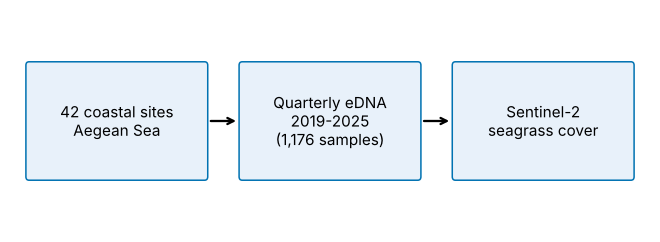
\includegraphics[width=0.8\linewidth]{figures/study_design.png}
  \caption{Study design: 42 sites, quarterly sampling 2019--2025, satellite cover from Sentinel-2.}
  \label{fig:design}
\end{figure}

\section{Results}
\begin{table}[h]
  \centering
  \begin{tabular}{lcc}
    \toprule
    Model & AUC (held-out sites) & Median lead time (years) \\
    \midrule
    eDNA early-warning & 0.91 & 2.1 \\
    Temperature only   & 0.68 & 0.4 \\
    \bottomrule
  \end{tabular}
  \caption{Early-warning performance on the 12 held-out sites.}
\end{table}
Eleven of the 14 sites that later lost more than 20\% cover showed the eDNA signal drop first.

\section{Limitations}
One sea, one seagrass species; satellite cover is itself an imperfect reference; the lead time
may shorten where turbidity limits eDNA persistence.

\section{Data availability}
Sequence data: ENA project PRJEB99999 (fictional). No code repository is released yet.

\bibliographystyle{plain}
\bibliography{refs}
\end{document}
